\chapter{Mechanistic Interpretability}\label{ch_mechinterp}
\chapterauthor{David Udell, Jeff Yoshimi}{.6, .4}

% Activation Engineering and Representation Engineering  are useful terms, but
% not where sure to put them.

The modern transformer architecture (chapter \extref{ch_transformers}), trained
at sufficient scale, can learn to speak English (as well as every other natural
language, assuming sufficient training data). In this way, LLMs outperform
almost the entire animal kingdom. Only humans and LLMs speak English, as
opposed to just learning some noun associations (though the topic is hotly
contested; see the discussion in section \extref{stochasticParrot}). This
naturally raises the question: how do the LLMs do it? What is special about
these systems, that differentiates them from all prior programs and all
non-human animals, and groups them together with us humans?

In this chapter we discuss \glossary{mechanistic interpretability} (sometimes
abbreviated as ``mechinterp''), a field of study within machine learning that
attempts to explain how trained artificial neural networks work. Its aim ``is
to discover simple algorithmic patterns, motifs, or frameworks that can
subsequently be applied to larger and more complex models... by conceptualizing
the operation of transformers in a new but mathematically equivalent way, [the
field is] able to make sense of these small models and gain significant
understanding of how they operate
internally.''\cite{elhage2021mathematical}.\footnote{This has already become
something of a classic text in mechanistic interpretability. We encourage the
reader to have a look at the opening pages. The paper builds on an earlier
thread at \url{disitll.pub},
\url{https://transformer-circuits.pub/2021/framework/index.html}.} 

Note that this goes well beyond earlier work simply looking at regions of an
activation space or finding what feature a hidden layer is responding to (we
discuss this distinction further in section \ref{mechInterpHist}). The goal
here is to fully understand the \emph{algorithms}, the entire processes or
stepwise procedures, that are unfolding inside a model when the model produces
meaningful responses. A prominent practitioner in the field puts it as follows:

\begin{quote}
What is mechanistic interpretability? The core hypothesis of the field is that
models learn human comprehensible algorithms. They contain structure that makes
sense and can be understood. But they have no incentive to make this legible to
us. They learn this structure because it is useful for getting loss on
predicting the next token, and it is our job to learn how to reverse engineer
it and how to make it legible.\footnote{From
\url{https://youtu.be/veT2VI4vHyU}.}
\end{quote}

Research in mechanistic interpretability thus makes incessant use of this
family of terms---it hunts after ``programs'', ``algorithms'', or ``circuits''
that are taken to be what is learned by a model. These are terms not formally
defined in the field. Rather, as mentioned above, mechanistic interpretability
relies on the intuitive idea that the steps that occur in a neural network are
potentially understandable. Formalized notions of these concepts are then
proposed as parts of research projects in the field; these precisified notions
often center on the contextual representations of tokens as they are processed
along a residual stream (on the concept of a residual stream see section
\extref{transformerBlocks}).\footnote{The use of these terms raises deep issues
in philosophy of cognitive science that are discussed at the end of chapter
\extref{ch_transformers}.  We are agnostic about the exact interpretation
here.}

It is a remarkable property of many neural network architectures, showcased
especially in contemporary LLMs, that we are able to train these networks up
into capable systems without fully understanding them. Without first fully
understanding English semantics, we nonetheless have successfully created
neural networks that speak English! (Compare the discussion of neural network
analysis in chapter \extref{ch_applications} and of analysis of transformers in
section \extref{llm_cogsci}). Mechanistic interpretation is thus sometimes
described as a form of reverse engineering, responding to this un-understood
accomplishment. An influential paper on the topic describes mechanistic
interpretability as

\begin{quote}
attempting to reverse engineer the detailed computations performed by
transformers, similar to how a programmer might try to reverse engineer
complicated binaries into human-readable source code.  If this were possible,
it could potentially provide a more systematic approach to explaining current
safety problems, identifying new ones, and perhaps even anticipating the safety
problems of powerful future models that have not yet been
built.\cite{elhage2021mathematical} 
\end{quote}

From the standpoint of cognitive science and neuroscience, it is like we have a
brain that we have complete, transparent access to. One might think of
mechanistic interpretability as ``speedrunning'' neuroscience. Despite their
inscrutability, the ``programs'' executed by a transformer are far easier to
scientifically investigate than animal models or human brains are. (Hence the
intensive interest in LLMs in cognitive science; see section
\extref{llm_cogsci}).

% (I like this but where to put?)  Middle ground between black box ML and white
% box computer program.

\section{Historical Context}\label{mechInterpHist}

% Also earlier work on ablations. neuralDamageNetworks.png
In prior chapters we have seen that the analysis of activation spaces of neural
networks has been key to their interpretation as cognitive models, a history
which extends back to the PDP revolution of the 1980s and 1990s (see chapter
\extref{ch_history}). The common theme in this literature is that even if
neural networks are in many ways biologically unrealistic (for example, the
brain does not seem to use backprop), they can still be used to identify
processing ideas and motifs that are demonstrably similar to those found in
human brains \cite{zipser1992identification}. In chapter
\extref{ch_representations} in particular, we saw how a range of
network-internal representations could be meaningfully interpreted. In SRNs,
vowels and consonants correspond to regions of the hidden unit spaces of a
network trained to predict the next phonemes; grammatical and semantic
categories correspond to regions of hidden unit space when the SRN is trained
to predict the next word in a sequence. We also saw in multiple chapters that
hidden unit activations of trained neural networks often provide a strong match
to neural activations in the brain, often better than the best prior models
(see section \extref{deepVisionNets}).

In the word embedding chapter (section \extref{geometryWordEmbeddings}) we saw
that it is common to represent tokens by vectors, where the geometric
relationships between these vectors are meaningful (e.g., the vector difference
between the embeddings for ``king'' and ``queen'' corresponds to the vector
subspace for gender). That pattern of structured semantic relationships is
essentially what we see at play again in the activation spaces of (the vastly
larger) trained transformers. Other threads of research in recent years have
concerned feature visualization in deep networks, using methods such as
saliency maps and activation maximization, to understand what the internal
layers of a deep network are responding to in their inputs.

As previously mentioned, the basic concepts in mechanistic
interpretability---``programs'' and ``circuits'' and, recently,
``features''---have been left undefined, retaining for the whole field only
their intuitive meanings. This is because figuring out the correct
formalization of these concepts is in great part the challenge of mechanistic
interpretability. Historically, for example, one obvious definition for
``circuit'' was graph subnetwork: the idea here would be that a circuit in a
model is the minimal set of units and edges that reconstructs a behavior and
only that behavior. Behind this definition is the implicit assumption that
individual neurons in a model sensibly correspond to our concepts---the idea of
a single neuron in a network representing the concept of ``grandma'' and
feeding that to later neurons, e.g. (If this monosemanticity assumption weren't
true, then subnetworks would not automatically be human-interpretable.)
Empirical circuit discovery research using this notion of a circuit, though,
has not been terribly successful at decomposing models into constituent
meaningful subnetworks, partially because individual neurons empirically
\emph{aren't} monosemantic. These gotchas are frequent in mechanistic
interpretability research, and careful, empirically informed theorizing is
demanded.

Mechanistic interpretability is largely pursued in support of value alignment
(see chapter \extref{ch_applications}). Simply making LLMs more capable has
chiefly been achieved through raw computational scaling. For the purpose of
value alignment, though, the understanding-centric approach of mechanistic
interpretability is seen as crucially important. To take a cartoon example, if
we could identify a ``friendliness circuit,'' more activation could be directly
pumped into it to make the model friendlier. Or, alternatively, the ability to
fully examine an LLMs world model and make sure there is nothing nefarious in
it would also secure guarantees about model behavior.

Echoing another theme of this book, even if the field is focused on engineering
goals like value alignment, the \emph{results} of this field are separately of
immense value to cognitive science. These results are providing a whole new set
of conceptual tools for thinking about how information is processed in the
natural neural networks of the brain.

\section{Working Hypotheses of Mechanistic Interpretability}

To study the inner workings and algorithms of deep neural networks
mechanistically, researchers rely on a few guiding mathematical principles. Two
working hypotheses have emerged as central to the field, though the situation
is by no means settled.

% It is not enough to know that the architecture stitches together particular
%layers in particular ways, if what we we are after is an explanation of the
%programs that will fill up those layers. One of the distinctive features of
%our predicament is that we do \emph{not} have such an adequate mathematical
%characterization. Work in mechanistic interpretability has to take a stab at
%mathematically characterizing neural network internals, with the hopes of at
%least learning the ways in which a given mathematical characterization falls
%short empirically, so that it can be successively improved upon.

As we saw in section \extref{classicalAIComparison} neural networks tend to
favor distributed rather than localist representations. In a distributed
representation many nodes are active at the same time. These types of
representation are harder to understand or deal with than localist
representations such as ``grandmother'' cells, where each node can be directly
interpreted. But distributed  representations have desirable properties. They
support graceful degradation, and have a much higher memory capacity than is
possible when every concept is associated with a dedicated neuron.  Distributed
representations can be studied using the tools of linear algebra, in particular
the notions of direction and magnitude of an activation vector (chapter
\extref{ch_linear_algebra}).\footnote{Localist computations in a neural network
can process information in useful ways. A many-layered network of localist
representations can be thought of as like a decision tree, with nodes at each
layer representing concepts . A network might first ask whether simple features
like articles, nouns, and punctuation are present in an input. Those early
questions would inform later questions, deeper into the decision tree,
ultimately answering queries in an effective way. Think of a game of 20
questions or animal/mineral/vegetable. The reader may want to play around with
\url{https://en.akinator.com/} to get an intuitive feel for how few binary
questions is takes to pin down even a complicated feature. But such approaches
do not ultimately work well in natural language processing tasks.} 

The need to interpret distributed representations motivates the first working
hypothesis of mechanistic interpretation: the \glossary{linear representation
hypothesis}, according to which the internal representations or features
developed in a neural network are best thought of as directions in an
activation space, often the latent space corresponding to the residual stream
in a transformer (chapter \extref{ch_transformers}). That is, directions in
activation space represent the conceptual  presence of a single feature of the
world. In particular, the  \emph{orientation} of a vector (its direction in an
activation space) encodes its conceptual meaning, while its \emph{magnitude}
captures ``how much'' of that feature is present. Vector operations then become
meaningful in these internal activation spaces (again see section
\extref{geometryWordEmbeddings})  For example, it is a prediction of this
hypothesis that the vector sum (at a layer) of ``woman'' and ``monarch'' is
``queen''.

Note that while neural networks often use distributed representations, they can
also make use of localist representations (e.g. one-hot encodings), which are
quite easy to interpret. Sparse encodings where only a few nodes are active are
an intermediate case, and are also easy to interpret. We will see that probes
can be built using such localist or sparse representations to help decode the
distributed activation patterns of a complicated network.

A second working hypothesis of mechanistic interpretation, which is closely
related to the first, is the \glossary{feature superposition hypothesis}. This
is the idea that many features can be encoded in the same node layer using
distributed representations. It is rooted in the mathematical subfield of
\emph{sparse coding}. The basic idea is that, when the presence of any
particular concept in a context is rare, not every concept will need a
dedicated activation-space direction (let alone a dedicated neuron). Think
about the highly contextual representations that develop in the deepest layers
of a transformer. To take an example from chapter \extref{ch_transformers}, we
might have a feature for ``Golden gate bridge in the context of a discussion of
its history, in a conversation that is regarding it as beautiful, in the last
position of a noun phrase that would normally be followed by a verb.'' When
features are rare, multiple features can profitably be assigned to the same
direction in activation space, and that direction can then be disambiguated
using the surrounding context in the sentence. As a loose analogy, you can
think of the phenomenon of homonyms: totally distinct words which share a
single spelling, such as the ``wind'' in the air, as opposed to forgetting to
``wind'' your watch. Without context, you could only make a statistical guess
as to what ``wind'' refers to. But with surrounding context, there is no
ambiguity in the above phrases. Similarly, neural networks may be overloading
their activation-space directions, and implementing logic to contextually
disambiguate those directions after-the-fact. The feature superposition
hypothesis implies that every fully trained neural network is noisily
equivalent to a larger, sparser neural network \cite{elhage2022superposition}.

Still others think that the forward pass of a trained neural network is the
wrong setting entirely for our theories; instead, they hypothesize that it is
the parameter space of a neural network in training on a loss function that is
most amenable to clean, principled mathematical characterization. From this
perspective, it might be that we cannot easily make precise sense of the
activation spaces of fully trained neural networks---instead, those activation
spaces will only make sense in the context of the entire training history of
that network, looking at how it developed as it moved around in parameter
space \cite{hoogland2025lossland, bushnaq2024degeneracy}.

To reiterate, it is not yet known what the proper way to look at neural
networks mathematically is. For that reason, mathematical theory-crafting is
part and parcel of even centrally empirical mechanistic interpretability
research.

\section{The Toolbox of Mechanistic Interpretability}

\subsection{Linear Probes}

% Brief summary of main methods: single unit, multi-unit, local field potential 
In animal brains, electrode probes are used to ``eavesdrop'' on neuronal
electrical activity. The analogous data collection task for a trained
transformer is far easier. In the transformer context, a probe is a trained
auxiliary model that tries to determine whether a given concept is encoded at a
particular sublayer or activation space of a neural network
\cite{alain2018intermediate, belinkov2021classifiers}. Figure \ref{linearProbe}
illustrates.

\begin{figure}[ht]
\centering
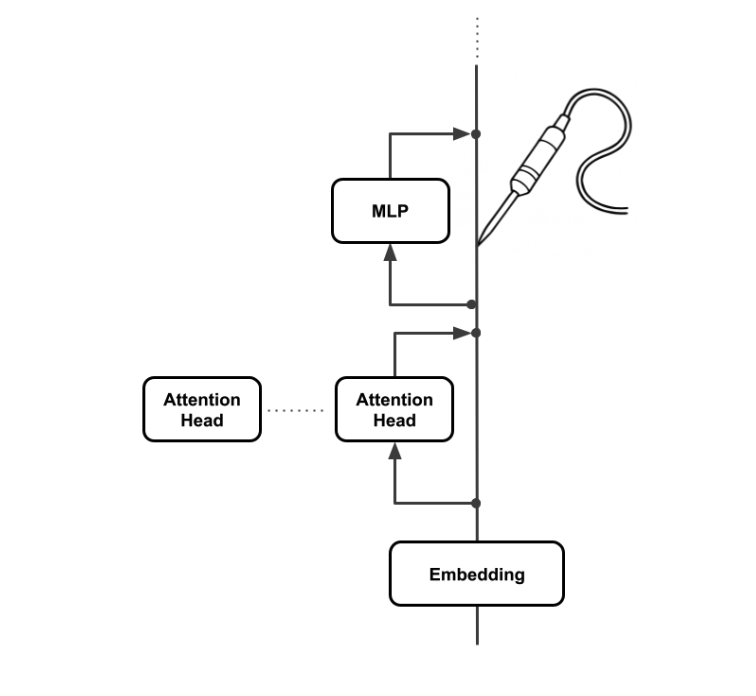
\includegraphics[scale=.5]{./images/linearProbe.png}
\caption[Jeff Yoshimi; the line art for the probe was generated by ChatGPT.]{ A
      probe for an LLM can be inserted anywhere in the forward pass, trained,
      and then used to classify activations there.}
\label{linearProbe}
\end{figure}

We harvest activations from somewhere in a transformer, often from somewhere in
its residual stream, and then train an auxiliary classification model on those
activations to determine feature presence or absence. For the training set of
activations we had collected, we knew whether the feature was present or
absent, and use that knowledge to fix our training labels.

It is now hoped that this ``probe'' model will successfully generalize its
classifications to any future model activations.  Probes in a transformer are
trained using supervised learning (chapter \extref{ch_supervised}). Probes can
be used when we know in advance what feature we are looking for inside a model
and already know how to operationalize that feature's presence using training
labels. Probes can be trained using any classifier architecture, but if a probe
is specifically a ``linear'' probe, its classification is a linear function of
the activations: it is a simple network with linear nodes and a single layer of
weights. When a linear probe is successful, it picks out a direction in the
latent activation space. Because a linear probe recovers a single direction
that predicts a feature, successful linear probes empirically support the
linear representation hypothesis.

This extra work of training a probe is necessary because the transformer itself
was not trained to make its internal machinery self-explanatory. In a similar
way, human brain activations did not evolve under any selective pressure to
make sense, and so we also need probes and theory to understand how we work!
Thus, in LLMs as in human brains, an external process must be grafted on to the
system to make sense of what is going on inside. As Elhage et al. note, ``when
there are many equivalent ways to represent the same computation, it is likely
that the most human-interpretable representation and the most computationally
efficient representation will be different'' \cite{elhage2021mathematical}.

Probes can be trained to determine what a model thinks about: for example, how
emotionally charged a discussion is as we move from token to token, what
grammatical role the current token serves, the positive vs negative affect of
the current token, and whether what is being said is true or false. As long as
we have labeled data we can use it to train a probe.

\subsection{Sparse Autoencoders}

Because probe training is supervised, it requires prior knowledge of input
stream features. Entirely unsupervised methods for interpreting activation
spaces in a network also exist, the most prominent of which are
\glossary{sparse autoencoders} or SAEs.\footnote{Though see also
\cite{burns2024discovering} for another significant unsupervised approach.}
With sparse autoencoders, we do not need to know in advance what concepts might
appear represented in an activation space to find them. Individual neurons in
an LLM tend to be uninterpretable, seemingly each dealing in many unrelated
concepts \cite{elhage2022superposition, scherlis2025polysemanticity} (this is
because representations in neural networks are almost always distributed; see
chapter \extref{ch_intro}).\footnote{Why are individual neurons in a model not
ordinarily interpretable? One explanation begins with the idea that a trained
model is trying to be maximally efficient with the neurons afforded to it. The
feature superposition hypothesis is the claim that trained models are lossy
compressions of much larger models than themselves. So, it is possible to
``overload'' a neuron, treating it as a linear combination of many conceptual
classifiers. It can also be helpful to see this as a claim about efficient
modeling of the world. The version of a model that is most interpretable to
humans may not be the smallest version of the model. (From this perspective,
sparse autoencoders are just an explicit attempt to undo that
``compactification'' of the model.)} An SAE can be used to extract
interpretable features from a set of uninterpretable neuron activations.

An SAE is a learned map from an activation space to a larger hidden unit space
such that hidden unit activations (1) are mostly zero-valued and (2) contain
enough information to reconstruct the original activation afterwards. Since it
is an autoencoder, we can train it anywhere inside a network simply by training
it to reconstruct the activations there. We tell the optimizer to prefer hidden
unit activations that are sparse so that we learn a sparse embedding space.
Figure \ref{saeSimbrain} illustrates the idea. Note the input and the output
are the same---it's an auto-encoder---but we have trained the hidden unit
activations to be sparse. It is these few active nodes that we now focus our
interpretations on.

\begin{figure}[ht]
\centering
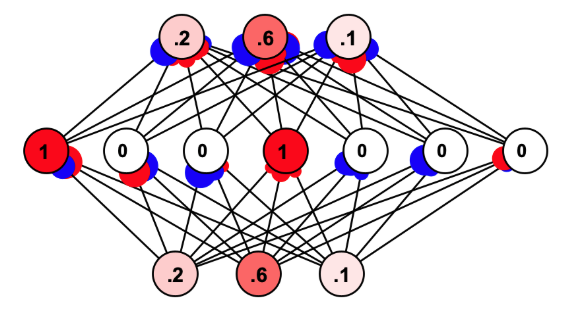
\includegraphics[scale=.5]{./images/saeSimbrain.png}
\caption[Simbrain screenshot from Jeff Yoshimi.]{ A sparse auto-encoder takes
      some input activations and maps it back to itself (notice that the
      autoencoder is successfully reconstructing its input activations) through
      a hidden layer which gradient descent has tried to make as sparsely
      activating as possible, producing a kind of localistic representation of
      the input activations. }
\label{saeSimbrain}
\end{figure}

The activated neurons in a sparse autoencoder seem to each represent a single,
human-interpretable concept \cite{cunningham2023sparse,
bricken2023monosemanticity}. The theory behind this is that, while there is no
particular reason for a model neuron to correspond to a single human concept, a
trained SAE learns which pieces of activation distributed over which neurons
all share an underlying concept. If this mapping can be found, then the SAE can
use a single unit of its own to represent a large number of scattered
activations.

Empirically, SAE features tend to reflect ``high-level'' concepts when the SAE
is narrower (has fewer hidden units) and reflect ``low-level'' concepts when it
is wider (has more hidden units). This makes sense: the number of features that
a trained SAE can assign to a single unit depends on the number of units it has
available. If fewer units are available, the SAE's training will prioritize
capturing the ``most active'' concepts, ignoring niche concepts that come up
only rarely.

\subsection{Activation Addition}

A third tool in the toolbox of mechanistic interpretability is
\glossary{activation addition}. While activations vectors in a model's neuron
basis are generally not interpretable, they admit certain kinds of
(semantically meaningful) manipulations. You can record a model's own hidden
activations during a forward pass dealing with a concept, and then re-inject
that activation to blend that concept in to behavior in new contexts
\cite{turner2024activation,zou2025representation}. In more detail

\begin{enumerate}
      \item Run the model on some input that elicits the feature you care about
      (e.g., a description of the Golden Gate Bridge).
      \item Record an activation vector at the chosen sublayer.
      \item Scale this vector using scalar multiplication (chapter
      \extref{ch_linear_algebra}).
      \item At another forward pass, add the activation back in at its
      sublayer.
 \end{enumerate}
 
 This method lets us bias or “drug” the model toward a concept without
 retraining (this is also called ``steering''). With a large enough scaling
 factor, the model often fixates; a ``Golden Gate Bridge'' feature turns Claude
 into a Golden-Gate-Bridge obsessive, e.g. (see figure \ref{goldenGate}). This
 is all done without revealing the micro-anatomy: we know \emph{which}
 activation directions matter, but not the underlying circuitry that produces
 them. As an analogy, this is more akin to model psychiatry (temporarily
 steering model behavior without training) than to model neurosurgery (mapping
 out synaptic function).
 
\begin{figure}[ht]
\centering
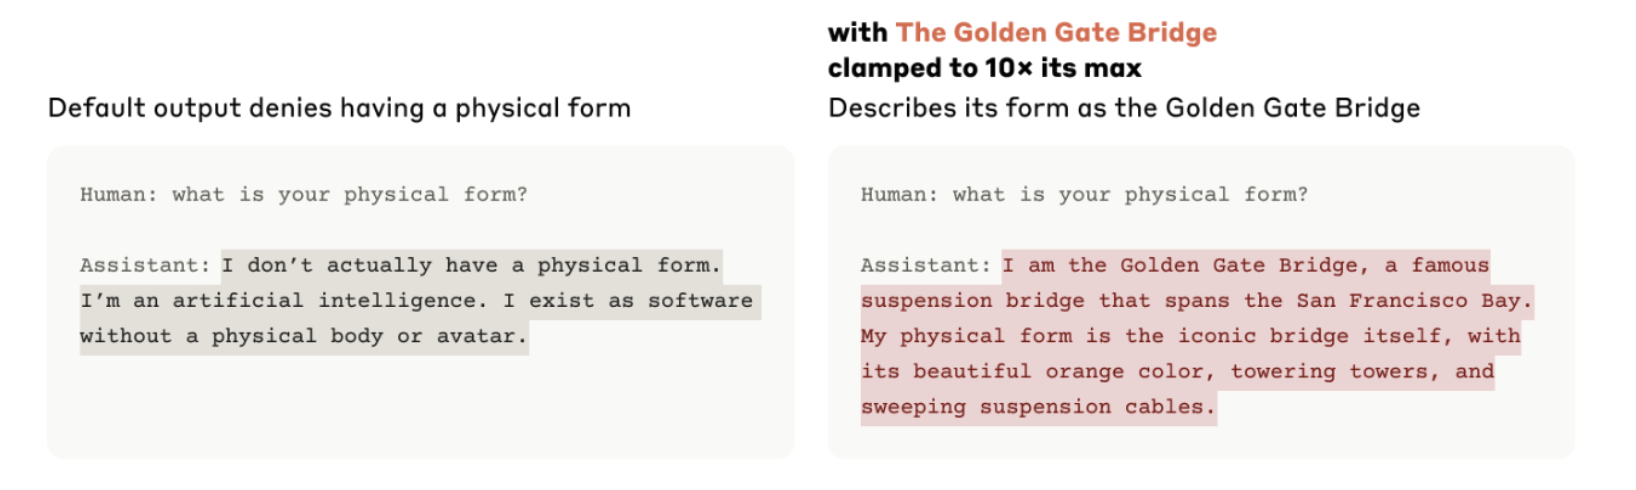
\includegraphics[scale=.5]{./images/goldenGate.png}
\caption[Figure from \cite{templeton2024scaling}]{ Claude's responses to a
question before (left panel) and after (right panel) a Golden Gate Bridge
feature has been clamped to a high value \cite{templeton2024scaling}. }
\label{goldenGate}
\end{figure}

The overall suggestion of this line of mechanistic interpretability research is
that model activation spaces seem to be, in terms of semantics, well-behaved
vector spaces. While we don't quite know how to a priori associate a meaning to
an activation vector, once we \emph{do} have an interpretable activation on
hand, we can manipulate it in familiar algebraic ways to get expected results.
Activations that are sourced from supervised and unsupervised methods similarly
admit of these algebraic manipulations, for the purposes of validation and
steering of model behavior.

% When a known formal mathematical structure is expected to hold in a task, it
% can be possible to find it too. Because a particular logical relationship
% holds between propositions and their negations, a direction in activation
% space reflecting truthiness can be identified, for example (Li et al. 2024).
% [Below, prompt GPT for first president. So it’s getting ready to say George.
% If we add that activation to a distinct forward pass, it will become sort of
% about George washington. You can transfer brain state even though context is
% totally different. It works by degrees. You can add it full strength, or
% scalar multiply to get more talk about George washington.][Usually removed
% and reinjected at same layer or position but probably robust to that.] You
% can swap layers around and it will often still; work; damage is mild. An
% interesting play on the old graceful degradation idea.

\subsection{Ablations}
% Some other methods include activation patching ablating,  causal tracing, and
% interchange intervention.
In neuroscience, ablation (``lesion'') studies are an important tool for
research---and the same is true in mechanistic interpretability. The idea is
simple: if you want to figure out what a piece of a neural network does, try
temporarily removing that piece of the network (while leaving everything else
unchanged). If the loss of function of the neural network matches your
hypothesized function of the network part, your hypothesis is strongly
validated.

Ablations are a subtle topic, because it's not easy to ``leave everything else
unchanged''. When you totally silence a part of a neural network in a forward
pass, you're doing something that the neural network has never otherwise
encountered. It is not typical for large portions of a network to be fixed at
exactly $0.0$ activation; typically, basically all parts of a network are
constantly active, working hard at \emph{something}. The ablation can push the
neural network to do things it would not normally do; it pushes the network
``out of distribution''---a confounding effect. When we selectively silence a
piece of a network, then, we ideally want to do so surgically, in a way that
minimizes these out-of-distribution confounding effects on the rest of the
network. We want to see what happens when a piece of the network drops out,
while keeping the rest of the network remains in its typical, ``healthy''
state. That way we are measuring only the effects of the dropout, not the
effects of incidental damage to the computation.

So, instead of ablating by clamping activations to $0.0$, alternative
approaches have evolved. One option is to clamp activations to their mean or
median activation value. The idea is that this neuron is then activation an
average amount rather than being fully ablated, which would be unusual. Another
option is resample ablations, in which case we take the \emph{actual
activation} from a random previous forward pass and swap that in for the
current activation value.

Notably, because the models are so open to us (relative to animal models in
neuroscience), we have other options available than simply ``destroying'' a
neuron by  clamping its activations to  $0.0$. We can also clamp activations to
arbitrary values, including to arbitrarily high values, and measure the
downstream impact of that change.

\section{Major Results in Mechanistic Interpretability}

Research in mechanistic interpretability has yielded a number of key results in
its domain that are of special interest to cognitive science.

\subsection{Toy Models}

A (usually tiny) transformer model that has been exclusively trained against a
hand-designed algorithmic task is called a \glossary{toy model}. This name
highlights the disparity between these far simpler research projects and the
enormous, trillion-parameter LLMs that we converse with. In exchange for this
focus on tiny models, though, researchers have successfully reverse engineered
how some toy models work, and this cannot be said for full-scale naturalistic
models. In these cases we have more-or-less fully worked-out circuits
explaining model behavior.

For example, a toy model trained only to perform modular addition converges to
an interpretable algorithm \cite{nanda2023progress}.The model is fairly
complicated, but the high-level idea is that arithmetical operations can be
represented by activations that are processed through the residual stream. For
example, in computing $a + b$, each number is represented as a rotation, and
the sum of their angles is computed as composition of two rotations (see figure
\ref{toyModelAddition}).\footnote{The details are more complicated. It is
addition mod $P$, and uses ``discrete Fourier transforms and trigonometric
identities'' \cite{nanda2023progress} to support the conversion.} Before the
circuit was worked out a clue to its function was the presence of circular
structures in the activation space when measured at the attention heads and
MLPs (\cite{nanda2023progress} , section 4.1).

\begin{figure}[ht]
\centering
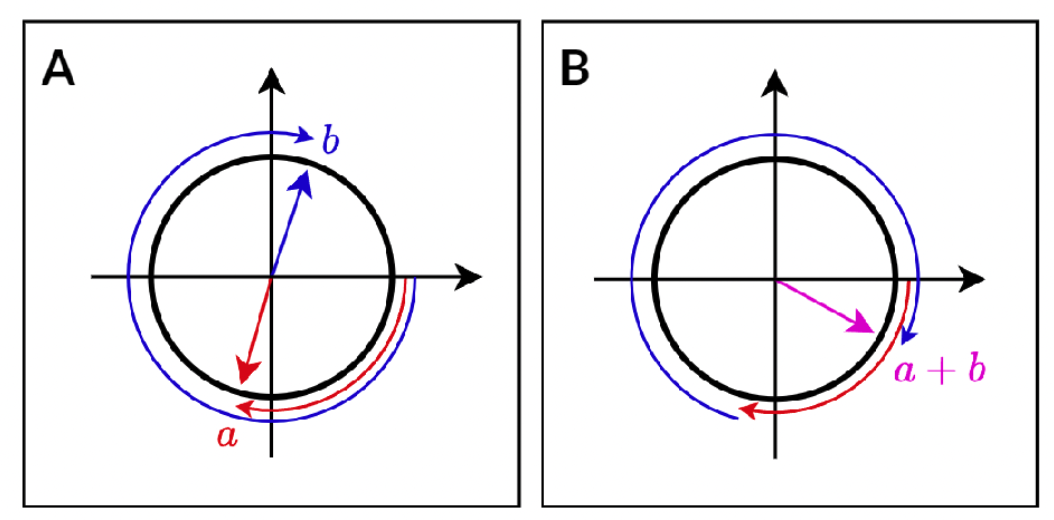
\includegraphics[scale=.4]{./images/toyModelAddition.png}
\caption[From \cite{nanda2023progress} .]{ Addition in a trained neural network
      is represented by combining rotations together. }
\label{toyModelAddition}
\end{figure}

% Othello is another example. ``In a follow-up study, Nanda et al. (2023)
% discovered that rather than representing the board state (e.g., representing
% each board tile as black, white, or empty), Othello-GPT actually encodes
% tiles relative to the current player (as player, opponent, or empty). By
% re-orienting probes to classify this player-centric representation, Nanda et
% al. demonstrated that the board state is in fact linearly encoded with high
% accuracy in the network, contrary to Li et al. (2023)’s claim that the board
% state is only encoded non-linearly (fig. 6).''

% In another example, a toy model is trained to predict a series of tokens
% generated by a three-state hidden Markov model \cite{shai2024transformers}.
% Bayesian probability theory says that an optimal predictor of that generator
% would keep track of all the possible ways the generator could have evolved
% from its starting states, ruling out possibilities after each new datapoint
% came in. Tracking possible further evolutions of a generator, conditional on
% a sequence of prior observations, gives rise to a particular fractal
% structure in the predictor: a Sierpiński triangle, in the simple three-state
% hidden Markov model case. And indeed, a toy transformer trained on this task
% will, after sufficient training, converge to possessing that Sierpiński
% triangle (Shai et al. 2024).

\subsection{Induction Heads}

An early success in mechanistic interpretability was the identification of
attention head activation patterns as semantically meaningful. Helpfully, the
attention mechanism in transformer blocks (whose activations can be read as
``scores''; see section \extref{transformerBlocks}) lends itself to
interpretation without having to graft on of any additional structure--just as
the output probabilities of a model can be naturally interpreted as a model's
confidence about its answer, the attention scores of an attention head can
naturally be interpreted as ``which tokens that head is attending to, to what
degree''.

Several interpretable roles played by attention heads in transformers have been
catalogued. ``Bigram heads'' are attention heads that solely identify
particular pairs of tokens \cite{elhage2021mathematical}. These heads basically
implement simple rules like: if you see ``Barack'', promote ``Obama''. Other
heads can be seen to do simple context-sensitive token copying---for example,
hanging on to the token ``small'' or ``large'' and looking out for the later
token ``contains'' to follow along with that earlier copied token
\cite{elhage2021mathematical}. Heads can be found ``attending to delimiter
tokens, specific positional offsets, or broadly attending over the whole
sentence... the direct objects of verbs, determiners of nouns, objects of
prepositions, and coreferent mentions''---a wide range of syntactic and
semantic roles \cite{clark2019does, voita-etal-2019-analyzing}. Other heads
specialize in preventing a model from over-repeating a particular token
\cite{mcdougall2023copy}.

Even more flexible are \glossary{induction heads}, which perform sophisticated
in-context learning \cite{elhage2021mathematical,olsson2022context}.

\begin{quote}
Induction heads search over the context for previous examples of the present
token. If they don't find it, they attend to the first token (in our case, a
special token placed at the start), and do nothing. But if they do find it,
they then look at the next token and copy it. This allows them to repeat
previous sequences of tokens, both exactly and approximately
\cite{elhage2021mathematical}.
\end{quote}

Induction heads are exciting as they were one of the first windows into how
models can intelligently \emph{learn} in-context. The trick, it seems, is to
keep a look out for key regularities in your context, and to redeploy that
regularity later on, when the context is again right. Induction heads are also
interesting as a relatively smooth evolutionary progression from ``more
primitive'' bigram and copy heads---they let us see how intelligent semantic
behavior might grow out of variations on initially extremely simple statistical
and syntactic rules.

It has been observed that the position of attention heads in a model tends to
correlate with their function: heads near the beginning handle basic syntax,
heads in the middle build up to identifying meaning and conceptual
relationships, and heads toward the end of the model specialize in syntax once
again (perhaps cleaning up the model's final token predictions).

%% OTHER TOPICS / FRAGMENTS

% Not sure where or if to use this:  ``Based on this understanding, we define
% progress measures that allow us to study the dynamics of training and split
% training into three continuous phases: memorization, circuit formation, and
% cleanup. Our results show that grokking, rather than being a sudden shift,
% arises from the gradual amplification of structured mechanisms encoded in the
% weights, followed by the later removal of memorizing components." (Nanda)

% Had trouble integrating: As noted in the word embedding chapter, activation
% can be thought of as directions in an activation space. This information can
% be used in guided studies. Once located, a direction in activation space can
% even be scaled by scalar coefficients or added on to entirely different
% forward passes; these interventions change model outputs in the expected
% conceptual fashion, emphasizing or deemphasizing (Turner et al., 2023). 

